\chapter{Proposed Solution}
\label{implementation}
\thispagestyle{plain}

In this Chapter, we describe the implementation aspects of the project. A general overview and service architecture is introduced in Section~\ref{subsubsec:service-architecture}. Section~\ref{sec:APNSIntegration} describes technical aspects of the Apple Push Notification Service (APNS), detailing some integration points for the proposed architecture. In Section~\ref{subsubsec:environment-configuration} we describe configurations used to improve the quality of the project's development process through the revision control system. Section~\ref{sec:prototyping} describes the developed prototypes for the mobile and Web applications.

\section{Service Architecture}
\label{subsubsec:service-architecture}
For the development of the project, we have used the following technologies:
\begin{itemize}
  \item MySQL~\cite{MySqlOrcale} - Service and Log Databases.
  \item Java Hibernate Framework~\cite{hibernate} - Service and Log~\gls{dal}s.
  \item Java Play Framework~\cite{playFramework} - REST API and Web application.
  \item Objective-C~\cite{ObjectiveC} - iOS Universal Application.
\end{itemize}
The presented technologies and frameworks were not studied during the curricular units of the Master's course. Regarding the MySQL technology, although it has not been studied, for used purposes it is very similar to Microsoft SQL Server~\cite{msSqlServer}, for the usage in this project.\\
\\
The main reason for choosing Java as the principal language instead of other technologies is the licensing costs associated to the development. The hibernate framework is licensed under the LGPL 2.1~\cite{licenseLGPG} and the Play Framework under the Apache License 2.0~\cite{licenseApacheV2}, with both allowing commercial and non commercial use of the components. The choice in developing the iOS application is due to technology popularity, its beautiful design, and the dynamics that can be achieved within this technology.\\
\\
\newpage
The GuideMe service architecture is depicted in Figure~\ref{fig:serviceArchitecture}.\\
\begin{figure}[h!]
 \centering
   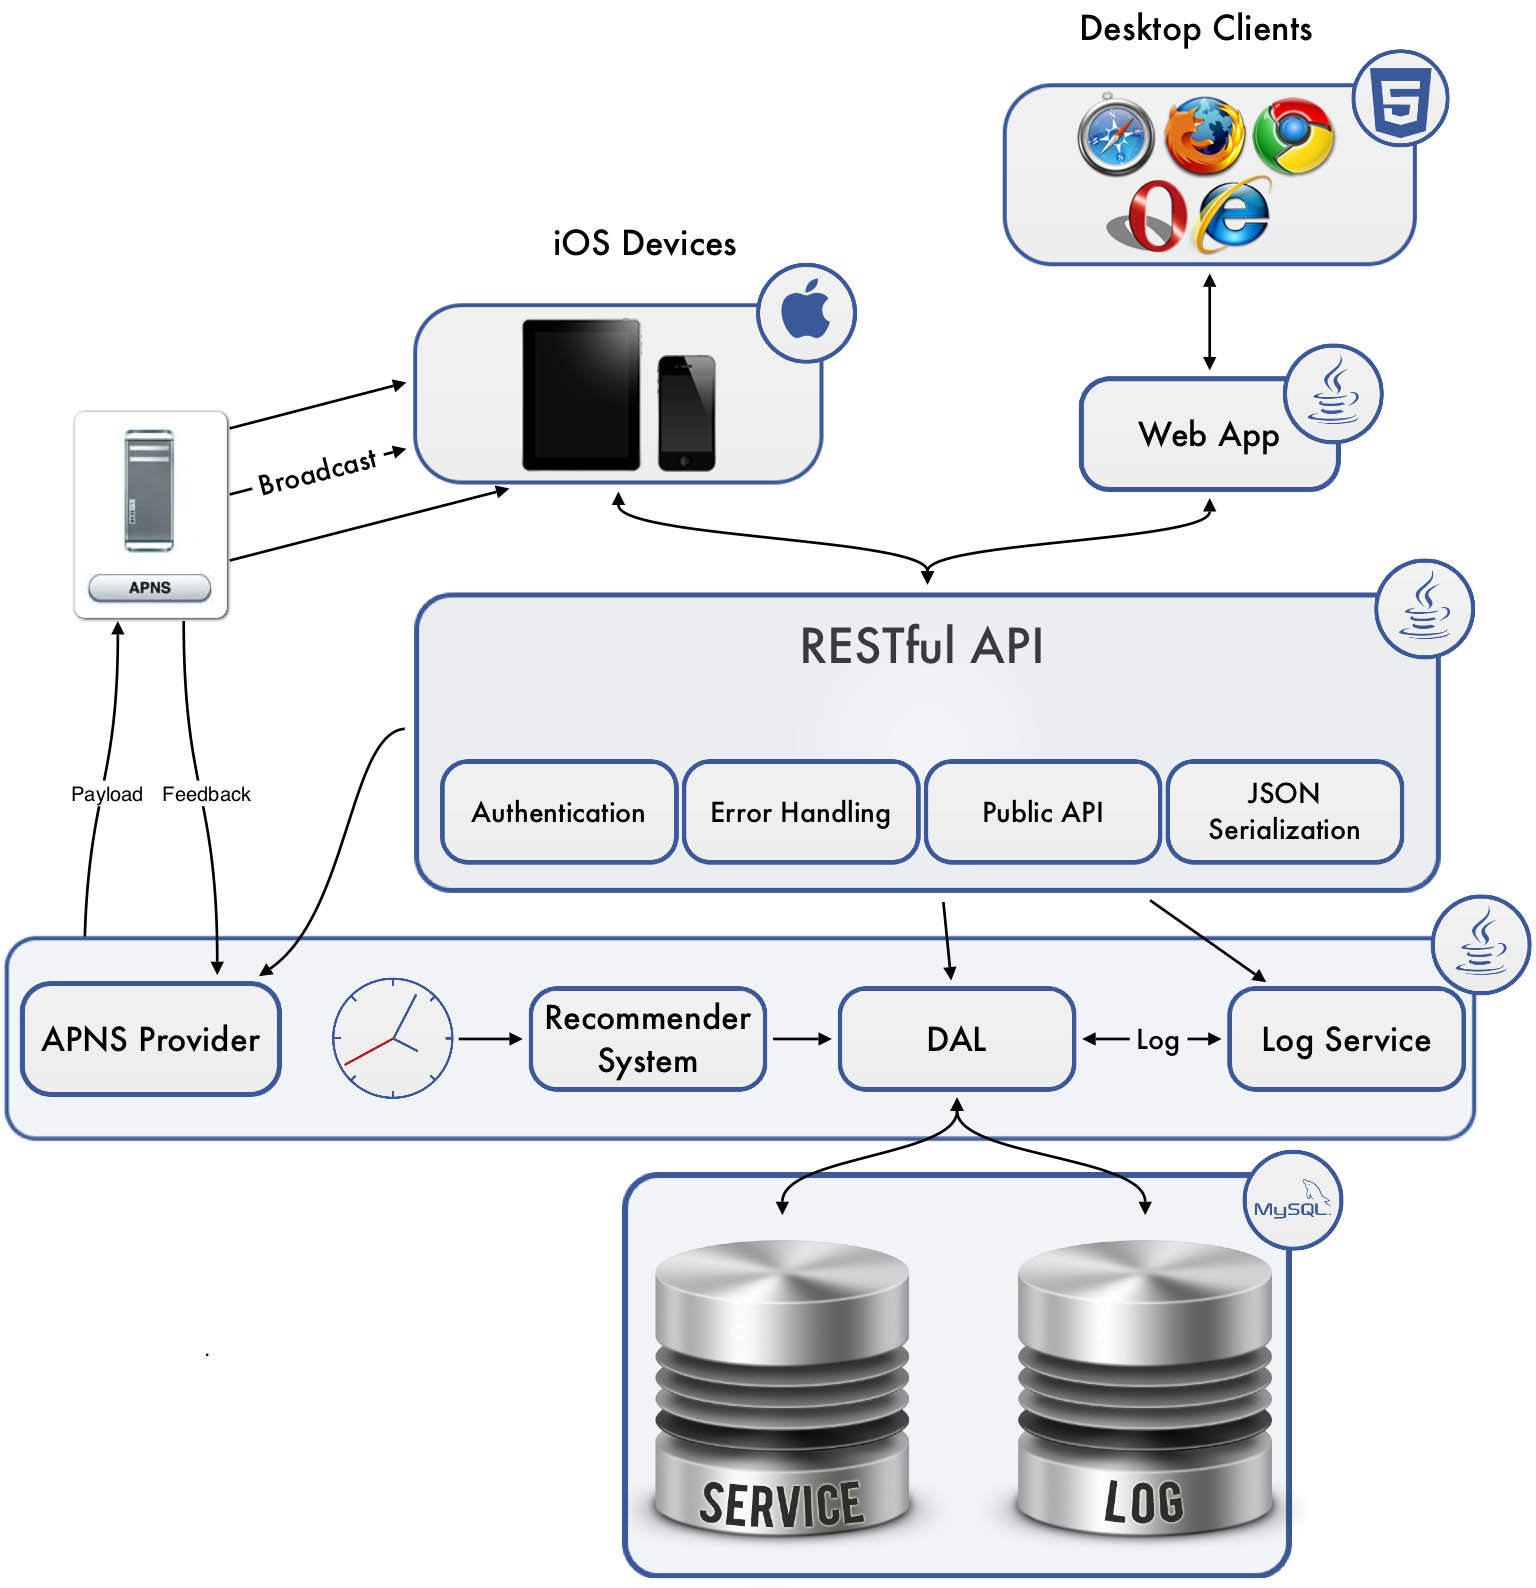
\includegraphics[width=12.5cm]{./images/diagrams/diagram_service_architecture.jpg}
   \caption{Detailed GuideMe service architecture.}
   \label{fig:serviceArchitecture}
\end{figure}\\
%%%%%%%%%%%%%%%
The purpose of each service component is as follows:
\begin{itemize}
\item Service Database - the main database, responsible for storing data regarding users, locations, among others.
\item Log Database - maintains log information about errors and warnings which may occur during the data retrieval or manipulation.
\\
\item Data Access Layer (DAL) - is responsible for communicating with the Service and Log database since each access to these storages is made through this component. 
\item Log Service - performs event logging by communicating with the DAL component.
\\
\item Recommender System - searches for new locations which can be recommended to users. This lookup process is triggered periodically by the configured Cron job.
\item RESTful API - provides a set of endpoints that can be accessed by different client applications, namely by the Web Application and mobile iOS devices.
\item \gls{apns} Provider - is responsible for sending push notifications to iOS clients in different occasions, for instance when new recommended locations are available.
\end{itemize}
%%%%%%%%%%%%%%%
To ensure the flexibility among the designed components, those were developed as a three tier architecture with the logical separation between the presentation, business logic, and database tiers. The adopted approach is shown on Figure~\ref{fig:threeTierArchitecture}.\\
\begin{figure}[h!]
 \centering
   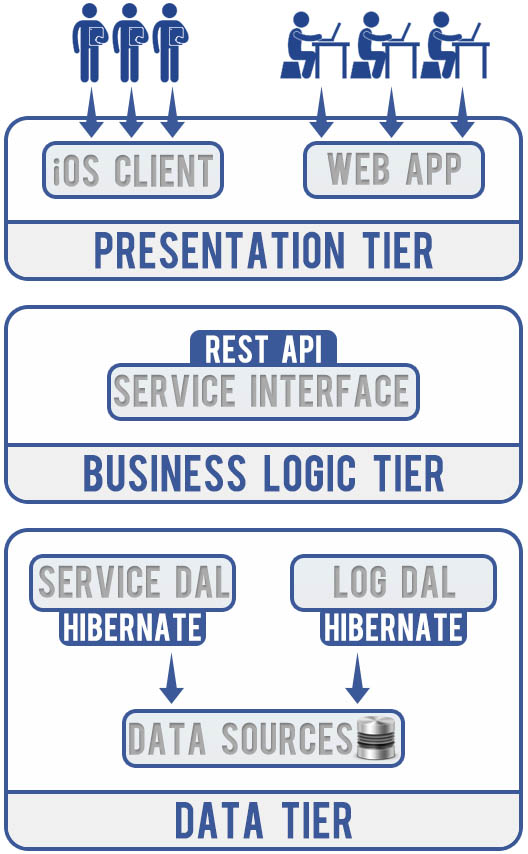
\includegraphics[height=8cm]{./images/diagrams/diagram_three_tier_architecture.jpg}
   \caption{Separation between service components as a three tier architecture.}
   \label{fig:threeTierArchitecture}
\end{figure}\\
The~\gls{treeTierDT} is responsible for storing and retrieving data from the database services. Exposes a set of interfaces that are used by the~\gls{treeTierBT}. The~\gls{treeTierBT} is responsible for controlling the service core functionalities by processing the client requests. The top most tier is the~\gls{threeTierPT} which represents the aggregation of various client applications that interact with the~\gls{treeTierBT} interface.\\
\\
The main benefits and drawbacks of the implemented architecture are as follows~\cite{threeTierArchitecture}:
\begin{itemize}
\item Benefits
	\begin{itemize}
		\item Scalability - The application servers for the \gls{treeTierBT} can be deployed on many machines where  the database connection is only required for each application server.
		\item Re-Use - The implementation aspects of the \gls{treeTierBT} are transparent to the PT, which have made 
  this layer more reusable.
		\item Security - When the \gls{treeTierBT} is located on separate application server from the DT, usually it is more secure and clients can't access the database directly.
	\end{itemize}
\item Drawbacks
	\begin{itemize}
		\item Complexity - it's more difficult to build a three tier architecture than other more simplistic solution.
	\end{itemize}
\end{itemize}
	
\section{Integration with the APNS}
\label{sec:APNSIntegration}
\gls{apns} is responsible for propagating information to iOS devices such as iPhone, iPod touch, and iPad. When a device connects to the Internet, it establishes an authorized and encrypted~\gls{ip} connection with the \gls{apns} and receives notifications over this persistent connection. If the application is not running, the user receives a notification on his devices~\cite{apns}.\\
\\
Figure~\ref{fig:apnsSimple} illustrates the simplified push notification path from an~\gls{apns} Provider to a client application, on the iOS device. The provider and the client application are the two parts which were developed in this project.\\
\begin{figure}[h!]
 \centering
   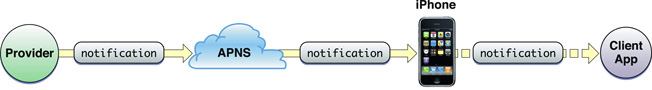
\includegraphics[width=12cm]{./images/diagrams/diagram_apns_simple.jpg}
   \caption{A push notification from a provider to a client application (adapted from~\cite{apns}).}
   \label{fig:apnsSimple}
\end{figure}\\
\\
In the following paragraphs, we provide a description of the main features and some \gls{apns} service implementation details.\\
\\
\textbf{Feedback Service}\\
When a user removes the application from the device, the Push Notification Service becomes unavailable for that user and the application in cause. The~\gls{apns} provides the feedback mechanism that allows detecting which devices are not receiving notifications. By using this information it is possible to filter which users the push notification should not be sent, thus minimizing the computation time and bandwidth usage.\\
\\
\textbf{Quality of Service}\\
The \gls{apns} guarantees that notifications are delivered to the user's device. When the device is offline or the user is unable to receive the notification, the~\gls{apns} service stores the notification. Later, when the device reconnects, the~\gls{apns} forwards the stored notification to the device. However, there are some limitations, only one notification per user is retained by the service and it remains for a limited time period before being removed.\\
\\
\\
\textbf{Security}\\
In order to establish communication between the provider and a device, the~\gls{apns} requires connection and token to be trustworthy. A connection between the~\gls{apns} and a provider is trusted if it is recognized by Apple, which has agreed to deliver notifications between the parties. After ensuring the connection trustworthiness, the ~\gls{apns} must guarantee that notifications are sent only to the intended device, and this is controlled by the device token which is requested during the client application startup. \\
\\
\textbf{The Notification Payload}\\
Each push notification carries a payload (maximum of 256 bytes) which represents the data to be downloaded to the client application. Any notification that exceeds this limit will be refused by the~\gls{apns}. Figure~\ref{fig:apnsPayload} represents the notification format.\\
%%%%%%%%%%%%%%%%%%
\begin{figure}[h!]
 \centering
   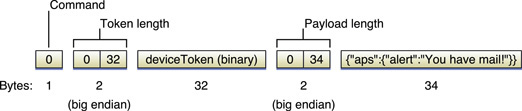
\includegraphics[width=12cm]{./images/diagrams/diagram_apns_payload.jpg}
   \caption{Notification Format (adapted from~\cite{apnsDetailed}).}
   \label{fig:apnsPayload}
\end{figure}
%%%%%%%%%%%%%%%%%%
\\
For each notification, a provider should compose in \gls{json}~\cite{json} format a dictionary named \emph{aps}. This dictionary should contain properties that specify the following actions~\cite{apns}: 

\begin{itemize}
\item an alert message to be displayed;
\item a badge number for the application icon;
\item a sound to be played when a notification is received.
\end{itemize}


\section{Environment Configuration}
\label{subsubsec:environment-configuration}
In this Section we describe the organization of the project and tools that have been used to improve the development process. Projects are hosted under the Git revision control~\cite{git} system using Bitbucket~\cite{Bitbucket} web-based hosting service. Table~\ref{tab:bitbucketRepositories} lists private repositories of the developed service components, and the base URL for all entries. The names under the \emph{Repository URL} column are prefixed with \url{https://aumanets@bitbucket.org/aumanets}.
\begin{center}
\begin{table}
    \centering
    \caption{Git repositories maintained in the Bitbucket service.} 
    \label{tab:bitbucketRepositories}
    \begin{tabular}{c}
	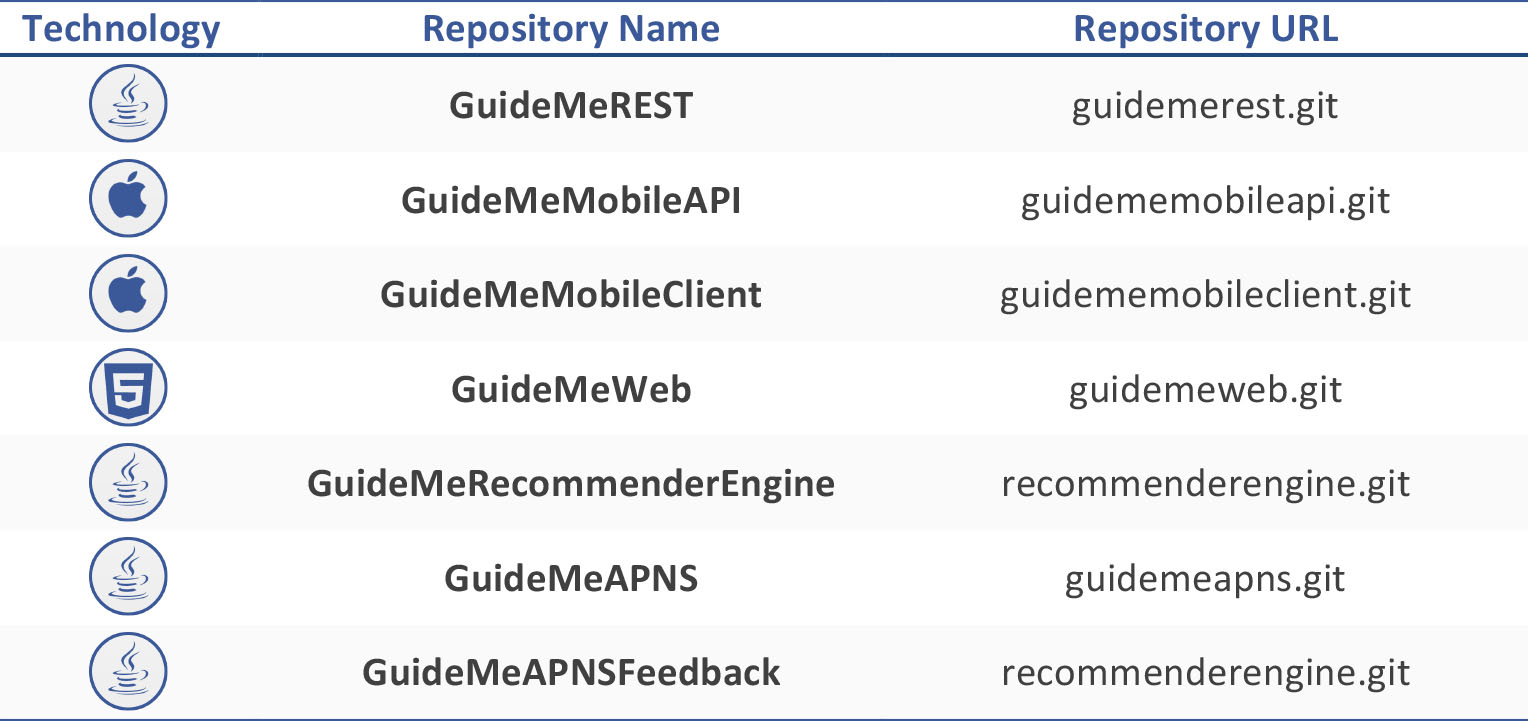
\includegraphics[width=12 cm]{./images/tables/table_bitbucket.jpg}    
    \end{tabular}
    \end{table}
\end{center}
%%%%%%%%%%%%%%%
The purpose of these repositories is as follows:
\begin{itemize}
\item \emph{GuideMeREST} repository stores the code of the \gls{rest} service and the DAL for the Service and Log databases. There is also a Section for the documentation with a description of the database model and detailed information regarding the organization of the tables. Some \gls{sql} scripts to create and populate the database model are also under this version control repository. For each component of this project a set of unitary tests was developed, allowing the verification of the correctness of the designed software modules.
%%%%%%%%%%%%%%%%%%%%%%%%
\item \emph{GuideMeMobileAPI} holds the source code of the developed framework which is used to access endpoints of the GuideMe REST API within iOS applications. It implements the wrappers for the JSON responses and the classes that allow to perform asynchronous requests in an organized way. There is a set of unitary tests for each remote operation responsible for validating the implementation of the REST API endpoints.
%%%%%%%%%%%%%%%%%%%%%%%%
\item \emph{GuideMeMobileClient} repository stores the source code of the iPhone and iPad application and also contains their initial prototypes. This project has a dependency with the \emph{GuideMeMobileAPI} repository.
%%%%%%%%%%%%%%%%%%%%%%%%
\item \emph{GuideMeWeb} is a repository for the Web-based application. It contains prototypes for different pages and the source code for both the user interface design (Twitter Bootstrap framework~\cite{twitterBootstrap}) and the server-side (Play framework~\cite{playFramework}).
%%%%%%%%%%%%%%%%%%%%%%%%
\item \emph{GuideMeRecommenderEngine} stores the source code of the implemented solution for the recommender system. The project contains the executable which is responsible for performing the recommendation computations and also a set of classes used to perform the evaluation of different~\gls{rs} implementations. It uses the GuideMeDAL in order to obtain users and locations for performing recommendations, as well as to store computed recommendations.
%%%%%%%%%%%%%%%%%%%%%%%%
\item \emph{GuideMeAPNS} holds the source code of the Java client for the Apple Push Notification service. The library aims to provide a highly scalable interface to the Apple server, while still being simple and modular; it was originally obtained from [6].
%%%%%%%%%%%%%%%%%%%%%%%%
\item \emph{GuideMeAPNSFeedback} repository with the Java project aimed to query the APNS Feedback service to consult iOS devices that are no longer able to receive Push Notifications. It uses the GuideMeDAL to update the database indicating the devices that should not receive push notifications.
\end{itemize}

\subsection{An Analysis of the REST API Frameworks}
Some \gls{rest} frameworks for the implementation of the services with Java environment, were analyzed, more specifically the Play~\cite{playFramework}, Restlet~\cite{restletFramework} and (JAX-RS) with Jersey~\cite{jaxRsJerseyExamples}\cite{jaxrsFramework}. Table~\ref{tab:javaRestComparison} shows a summarized comparison of these frameworks stating their key benefits and drawbacks.
%%%%%%%%%%%%%%%
\begin{center}
\begin{table}
    \caption{Comparison of three popular Java REST frameworks.} 
    \label{tab:javaRestComparison}
    \begin{tabular}{c}
	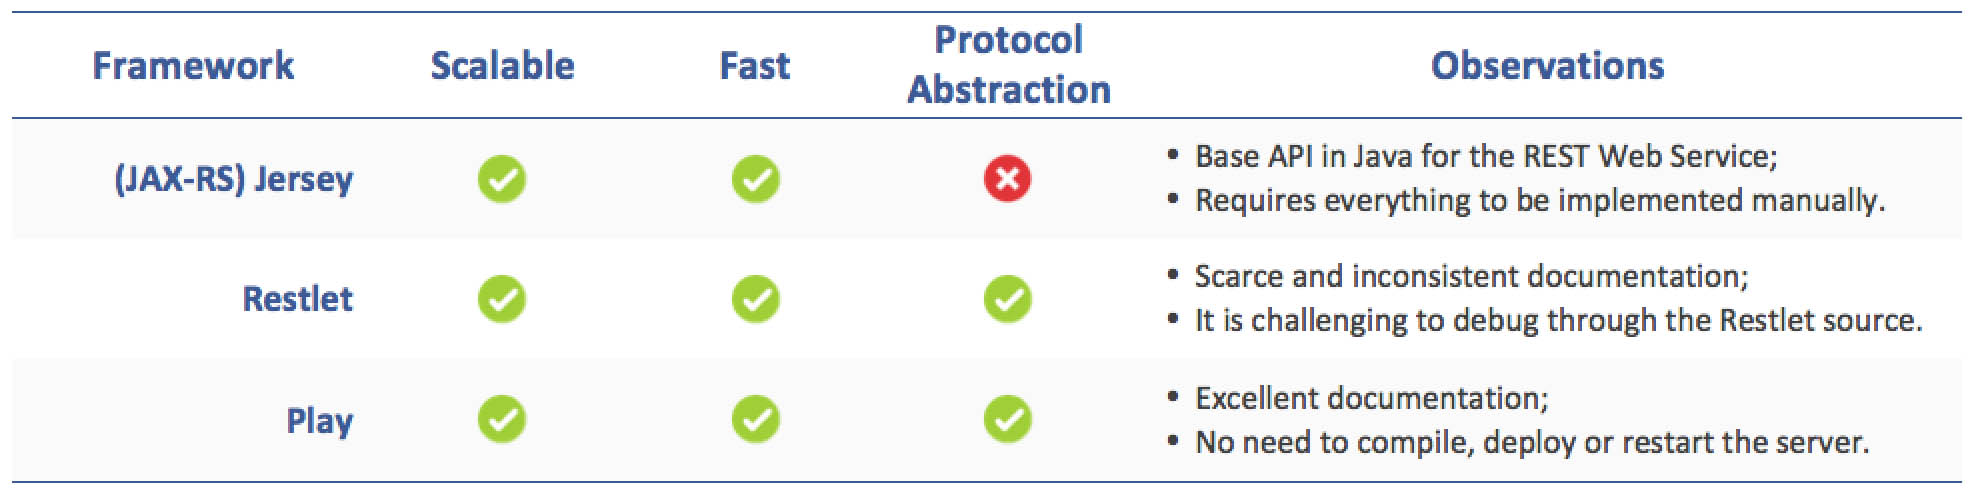
\includegraphics[width=14.7 cm]{./images/tables/table_java_rest_framework_comparison.jpg}    
    \end{tabular}
    \end{table}
\end{center}
%%%%%%%%%%%%%%%
Among these frameworks, the preferred choice is the Play framework which fulfills all requirements and has the highest number of benefits for the development process, as compared to the other two approaches.\\
\\  
\subsection{Web Application Development Technologies}
For the development of the web application, some programming languages and frameworks were studied. Initially, PHP~\cite{php} was the preferred language, but it has presented some problems and disadvantages, as compared to other approaches. As a script language, PHP is easy to learn but it lacks standards and conventions and it has earned a kind of bad reputation over the past years~\cite{phpBadReputation}. There is a lot of bad code and malformed examples that may lead to problematic solutions. The code is difficult to read and to maintain.\\
\\
Web development with the Play Framework presents more benefits than PHP. It was designed to emphasize productivity. This framework comes with powerful Scala-based template engine~\cite{playFramework}. The key advantages of the Play Framework, that are not easily achieved in PHP are as follows:
\begin{itemize}
\item Elegant URL design - flexible \gls{url} configuration without framework-specific limitations. For example \url{http://someurl/item?id=1} or \url{http://someurl/item/1}.
\item Template system  - extensible and designer-friendly template language that separates the design from content and Java code.
\item Internationalization - full support for multi-language applications, which allows to specify translation strings and provides hooks for language-specific functionality.
\end{itemize}
%%%%%
%%%%%
\subsection{Data Access Layer Frameworks}
The~\gls{dal} is implemented using the Hibernate~\cite{hibernate} framework for Java. Hibernate is an~\gls{orm} library that provides a framework for mapping an object-oriented domain model to a relational database, which makes the data access more abstract and portable, as compared to the traditional \gls{jdbc} approach. There are many other \gls{orm} frameworks (ActiveJDBC~\cite{activeJDBC}, jOOQ~\cite{jooq}, among others), but the Hibernate has a large community and currently is the most widely used by developers. Greater tool support is an important aspect, because eases the task of finding solutions to software problems. These and the following advantages justify our decision in adopting Hibernate as the~\gls{orm} framework.\\
\\
The main advantages of the Hibernate framework are as follows~\cite{hibernateBenefits}:
\begin{itemize}
\item Performance - generates efficient queries and employs first and second level caching strategy. The first level caching refers to the actions associated with the context of the current session, while the second level caching refers to the entire application. Both strategies are designed to minimize the number of ~\gls{sql} queries that are executed over the database.
\item Effective Cross-Database Portability - supports portability across different relational databases. The framework allows to easily configure its dialect, being independent of the database concrete functionalities, it specifies which \gls{sql} language should be used with the database. With this feature, it is easy to migrate to another relational database engine, if needed. 
\item Developer's Productivity - it has a short learning curve. It creates a clear abstraction level between the Java objects and the database model.
\end{itemize}

%%%%%
%%%%%

%%%%%%%%%%%%%%%%%%%%%%%%%%%%%%%%%%%%%%%%%%%%%%%%%%%%%%%%%%%%
\section{Prototyping}
\label{sec:prototyping}
In this Section we describe the designed prototypes that have facilitated the developments of the Web and iOS applications. The complete set of prototypes can be found in the corresponding repository of the application in cause.
%%%%%%%
%%%%%%%
\subsection{Web Application}
\label{subsec:WebAppPrototype}
Using the Adobe Photoshop~\cite{photoshop} software, a set of prototypes was created for the Web application, representing its most important features. The prototypes can be found int the \verb"GuideMeWeb" repository and they already implement the desired look and feel for this application. Each prototype provides the specification of the page \gls{url} and some notes regarding the specific actions. An example of the designed prototypes is shown on Figure~\ref{fig:guideMeWebScreenshots}. Figure~\ref{fig:guideMeWebScreenshots}~(\subref{fig:guidemeWebScreenshots1}) shows the page with the touristic locations that the user wants to visit, with the recommended locations displayed under the navigation menu. The prototype on Figure~\ref{fig:guideMeWebScreenshots}~(\subref{fig:guidemeWebScreenshots2}) illustrates the page with the location details, where the most important information regarding the chosen touristic locations is shown, such as: map with the location coordinates, average rating, preferred time of the visit, weather conditions, among others.\\
\begin{figure}
        \begin{subfigure}[b]{0.5\textwidth}
                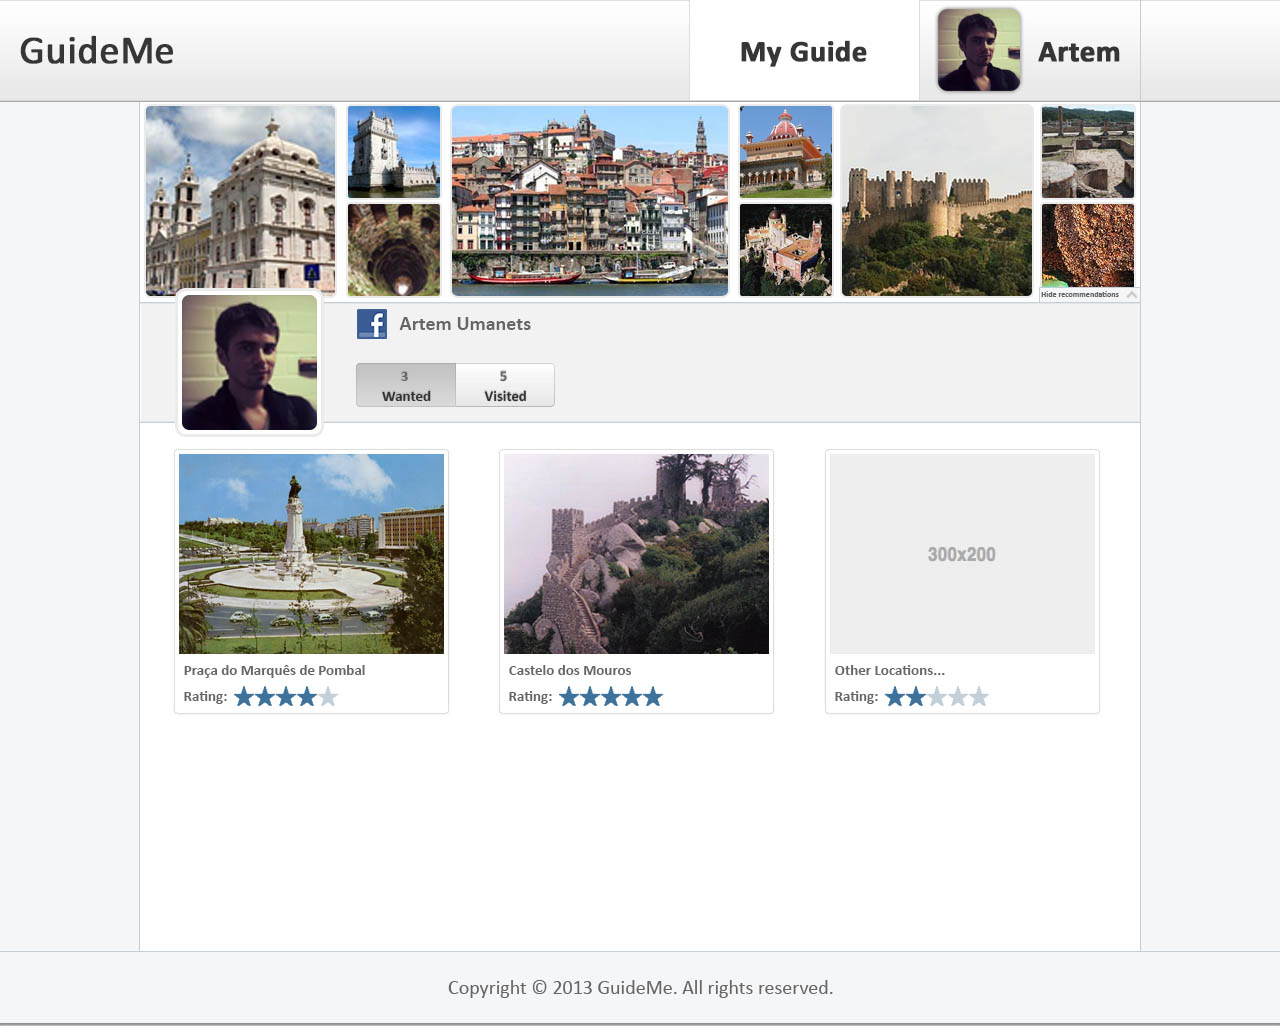
\includegraphics[height=5.8cm]{./images/screenshots/screenshot_prototype_web_1.jpg}
                \caption{Wanted locations.}
                \label{fig:guidemeWebScreenshots1}
        \end{subfigure}%
        \begin{subfigure}[b]{0.5\textwidth}
                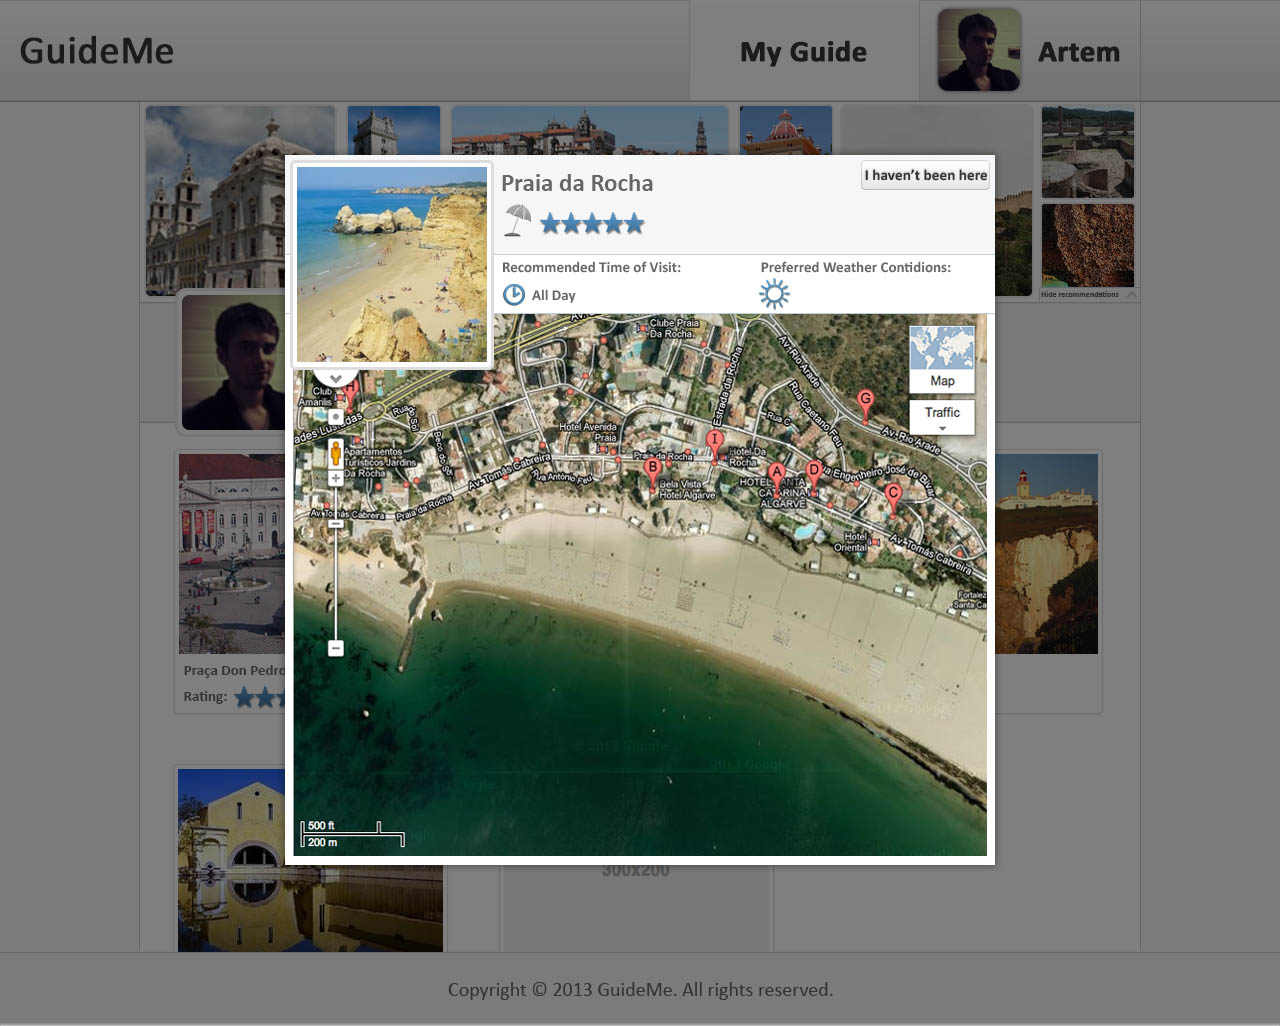
\includegraphics[height=5.8cm]{./images/screenshots/screenshot_prototype_web_2.jpg}
                \caption{Location details.}
                \label{fig:guidemeWebScreenshots2}
        \end{subfigure}
        \caption{GuideMe Web application prototypes.}
        \label{fig:guideMeWebScreenshots}
\end{figure}
\\
The hierarchy of the main operations of the Web application is shown on Figure~\ref{fig:webSiteHierarchy}. The \emph{Admin} users have access to the whole application while \emph{Standard} users have the same permissions, except to consult the API Documentation.
%%%%%%%
\begin{figure}[h!]
 \centering
   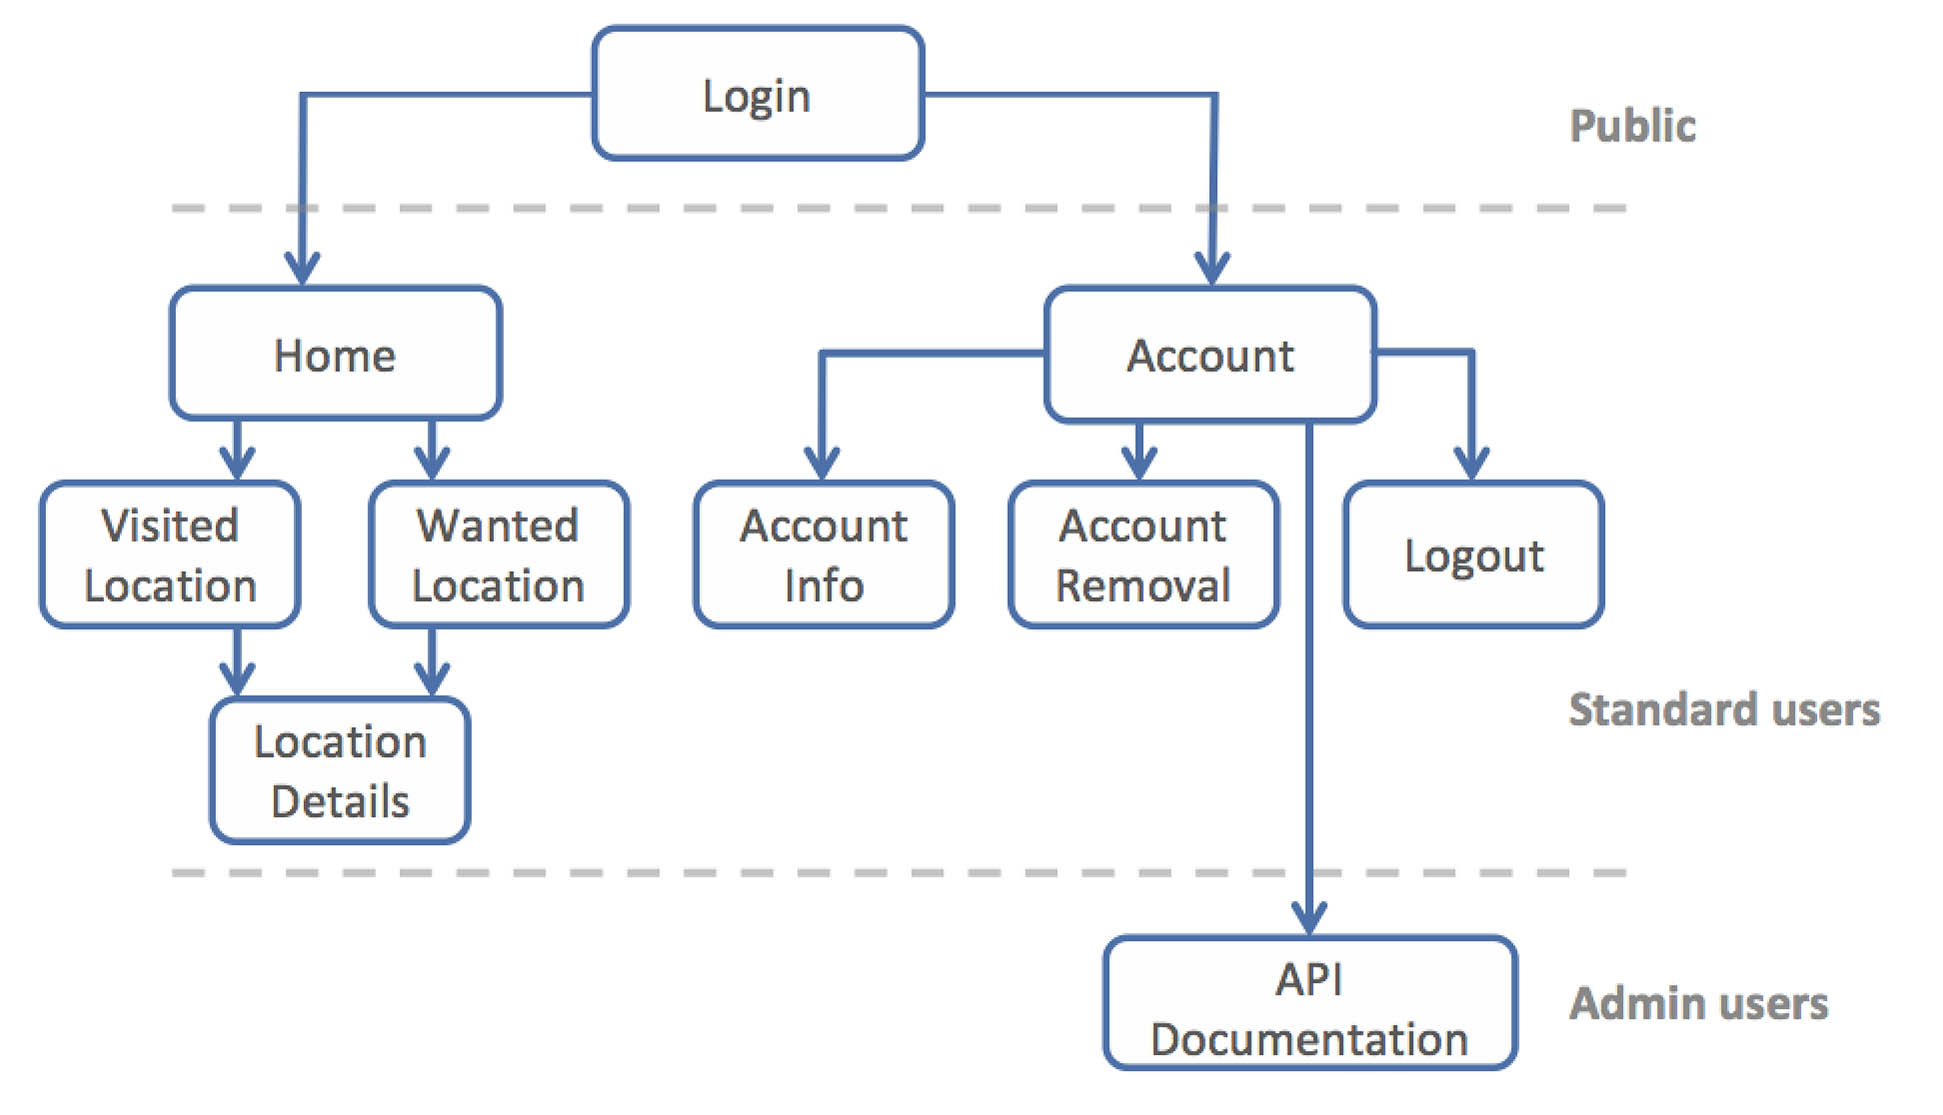
\includegraphics[height=5.5cm]{./images/diagrams/diagram_hierarchy_web.jpg}   
   \caption{Hierarchy of the supported operations within the Web application.}
   \label{fig:webSiteHierarchy}
\end{figure}
%%%%%%%
\subsection{iPhone Application}
\label{subsec:iPhoneApp}
A set of prototypes for the iPhone application was designed using the Adobe Photoshop and the AppCooker~\cite{appCooker} application for the iPad. The complete designs can be found in the \verb"GuideMeMobile" repository. Some screenshots of the designed prototypes are shown on Figure~\ref{fig:guideMeScreenshots}.\\
\\
\begin{figure}
        \centering
        \begin{subfigure}[b]{0.25\textwidth}
                \centering
                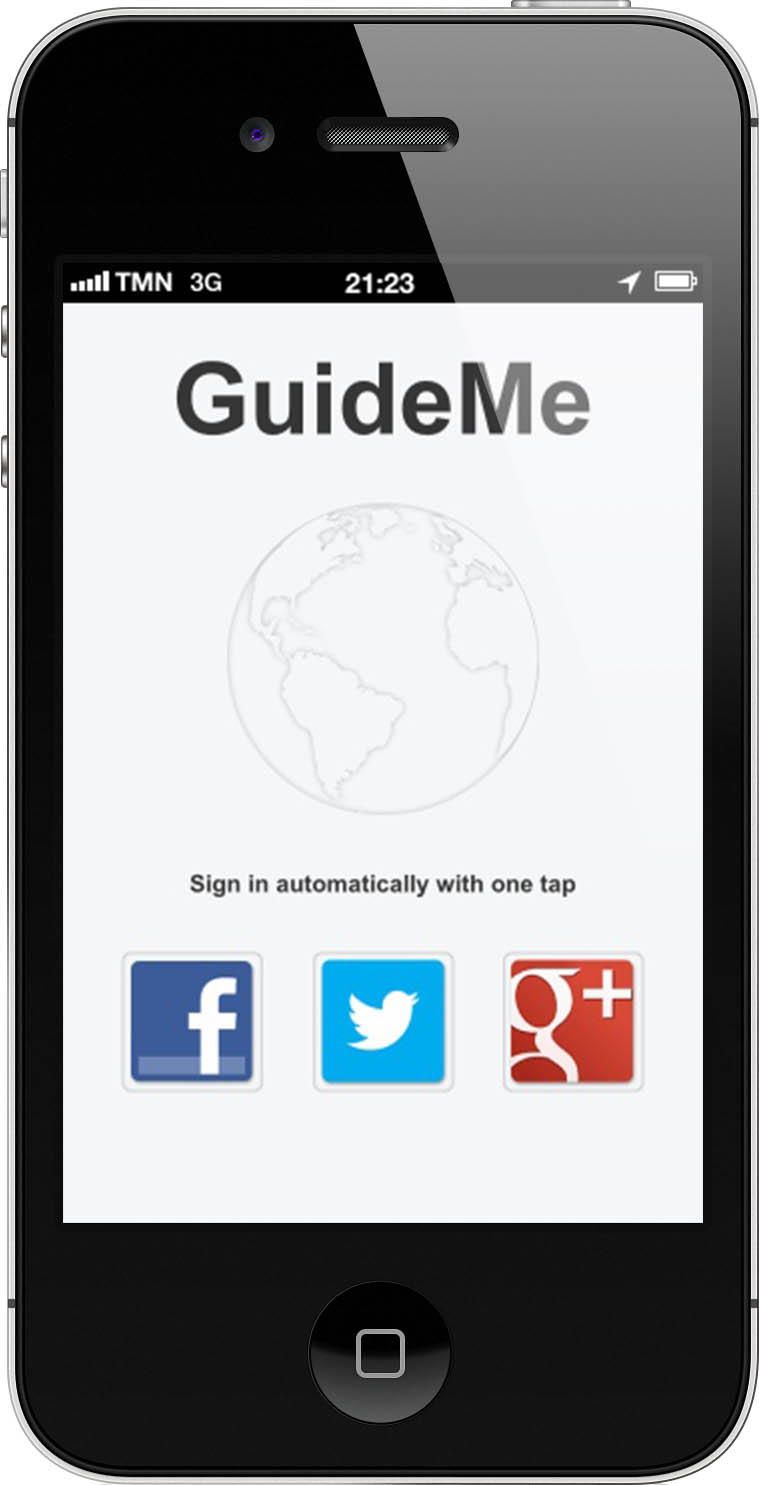
\includegraphics[height=7.0cm]{./images/screenshots/screenshot_prototype_mobile_1.jpg}
                \caption{Login screen.}
                \label{fig:guidemeiPhoneScreenshots1}
        \end{subfigure}%
        \qquad
        \begin{subfigure}[b]{0.25\textwidth}
                \centering
                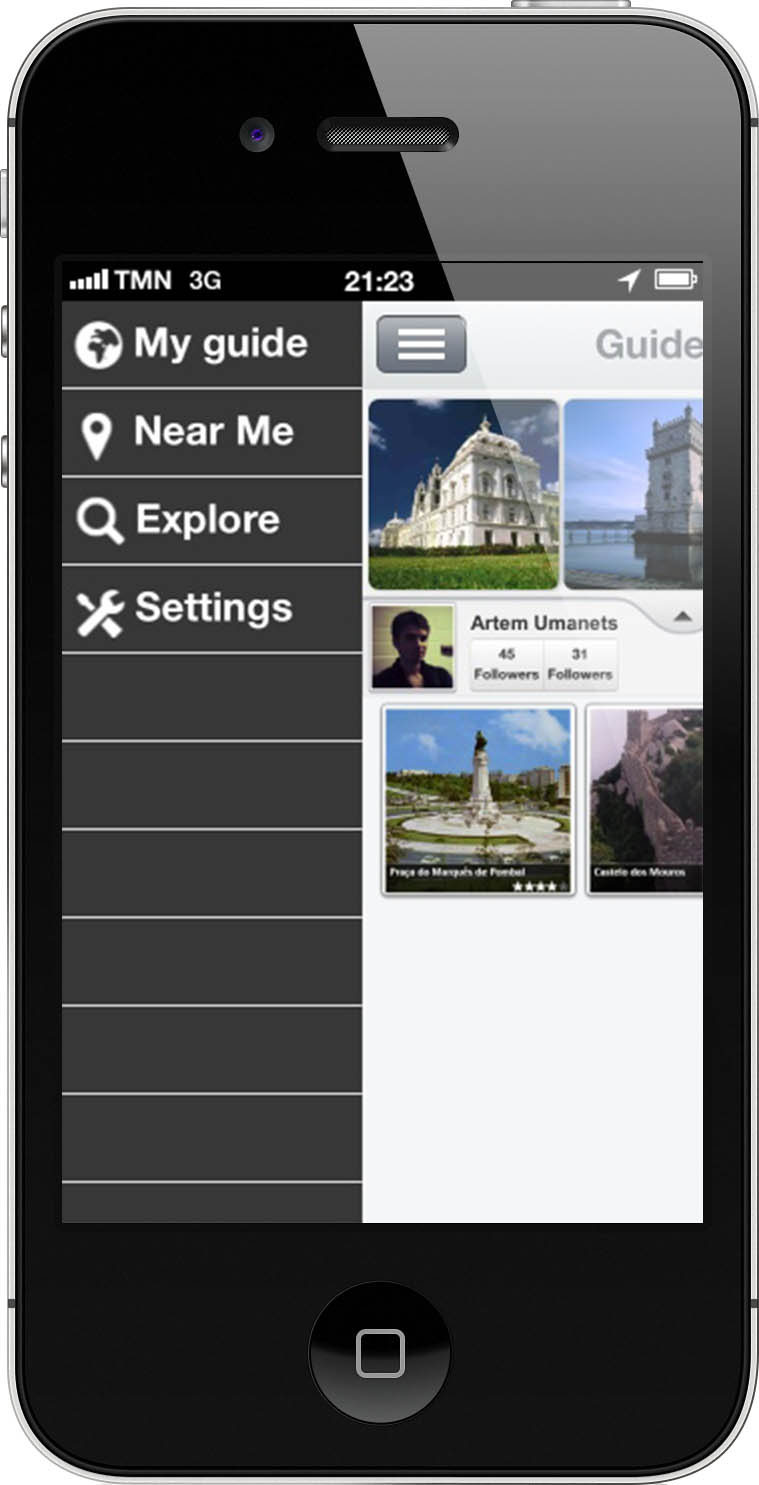
\includegraphics[height=7.0cm]{./images/screenshots/screenshot_prototype_mobile_2.jpg}
                \caption{Menu options.}
                \label{fig:guidemeiPhoneScreenshots2}
        \end{subfigure}
        \qquad
        \begin{subfigure}[b]{0.25\textwidth}
                \centering
                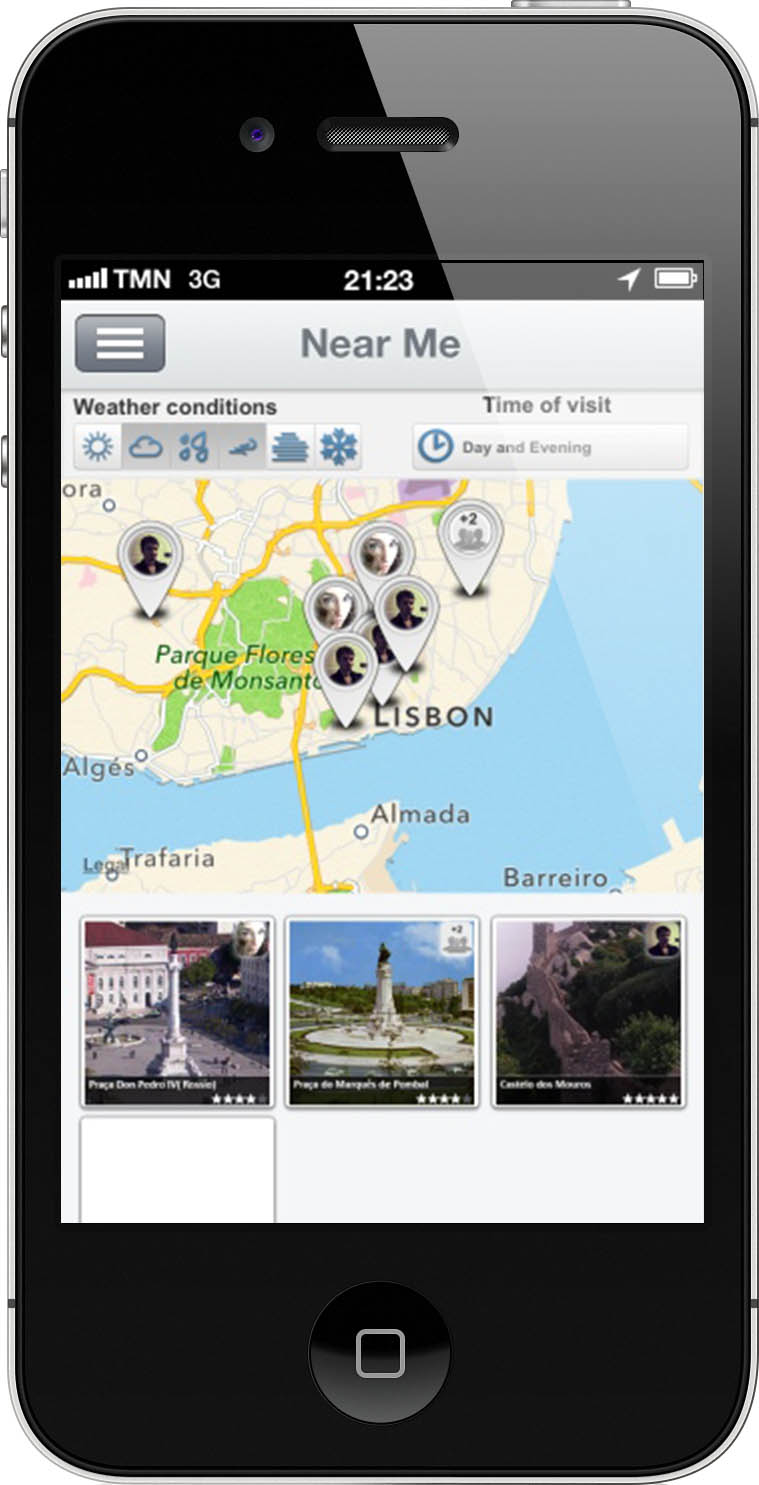
\includegraphics[height=7.0cm]{./images/screenshots/screenshot_prototype_mobile_3.jpg}
                \caption{Nearby locations.}
                \label{fig:guidemeiPhoneScreenshots3}
        \end{subfigure}
        \caption{Screenshots of the GuideMe application for the iPhone.}
        \label{fig:guideMeScreenshots}
\end{figure}
\\
Figure~\ref{fig:guideMeScreenshots}~(\subref{fig:guidemeiPhoneScreenshots1}) shows the authentication screen, where users are able to perform login by using the preferred social service (e.g. Facebook, Twitter, or Google+). Figure~\ref{fig:guideMeScreenshots}~(\subref{fig:guidemeiPhoneScreenshots2}) illustrates the main screen with the expanded navigation menu, which allows the navigation through the different parts of the application. This kind of navigation could be implemented using the Toolbar (usually located at the bottom of the screen) component but the presented choice offers more benefits by providing more space to be filled with the information about the touristic locations. The recommended locations are presented above the users photography. Figure~\ref{fig:guideMeScreenshots}~(\subref{fig:guidemeiPhoneScreenshots3}) shows an example of the \textbf{Near Me} feature, which consists in showing the touristic locations near the user's current location. On the top part of the screen, it is possible to configure filtering options, by specifying the weather conditions and the preferred time of visit. Through the map, users can visualize touristic locations, places where they have been, and other locations visited by their friends.\\
\\
Figure~\ref{fig:iosStandardUserHierarchy} illustrates the hierarchy of the operations that can be performed by standard users, where \emph{Explore}, \emph{My Sights}, and \emph{Friends} represent the main sections of the application. Users with the \emph{Admin} privileges have access to an additional section that is not visible to \emph{Standard} users.\\
\\
Each section is detailed as follows:
\begin{itemize}
\item Explore - presents a list of sights, filtered by the following criteria:
  \begin{itemize}
    \item select the attraction, country, city or user's current location.
    \item choose preferred weather conditions and time of day.
    \item specify the user's available time.
    \item search with custom description.
  \end{itemize}
\item My Sights - used to consult the visited, wanted, or recommended touristic locations.
\item Friends - offers the possibility to consult the followed users and to search for new users.
\end{itemize}
%%%%%%%
\begin{figure}[h!]
 \centering
   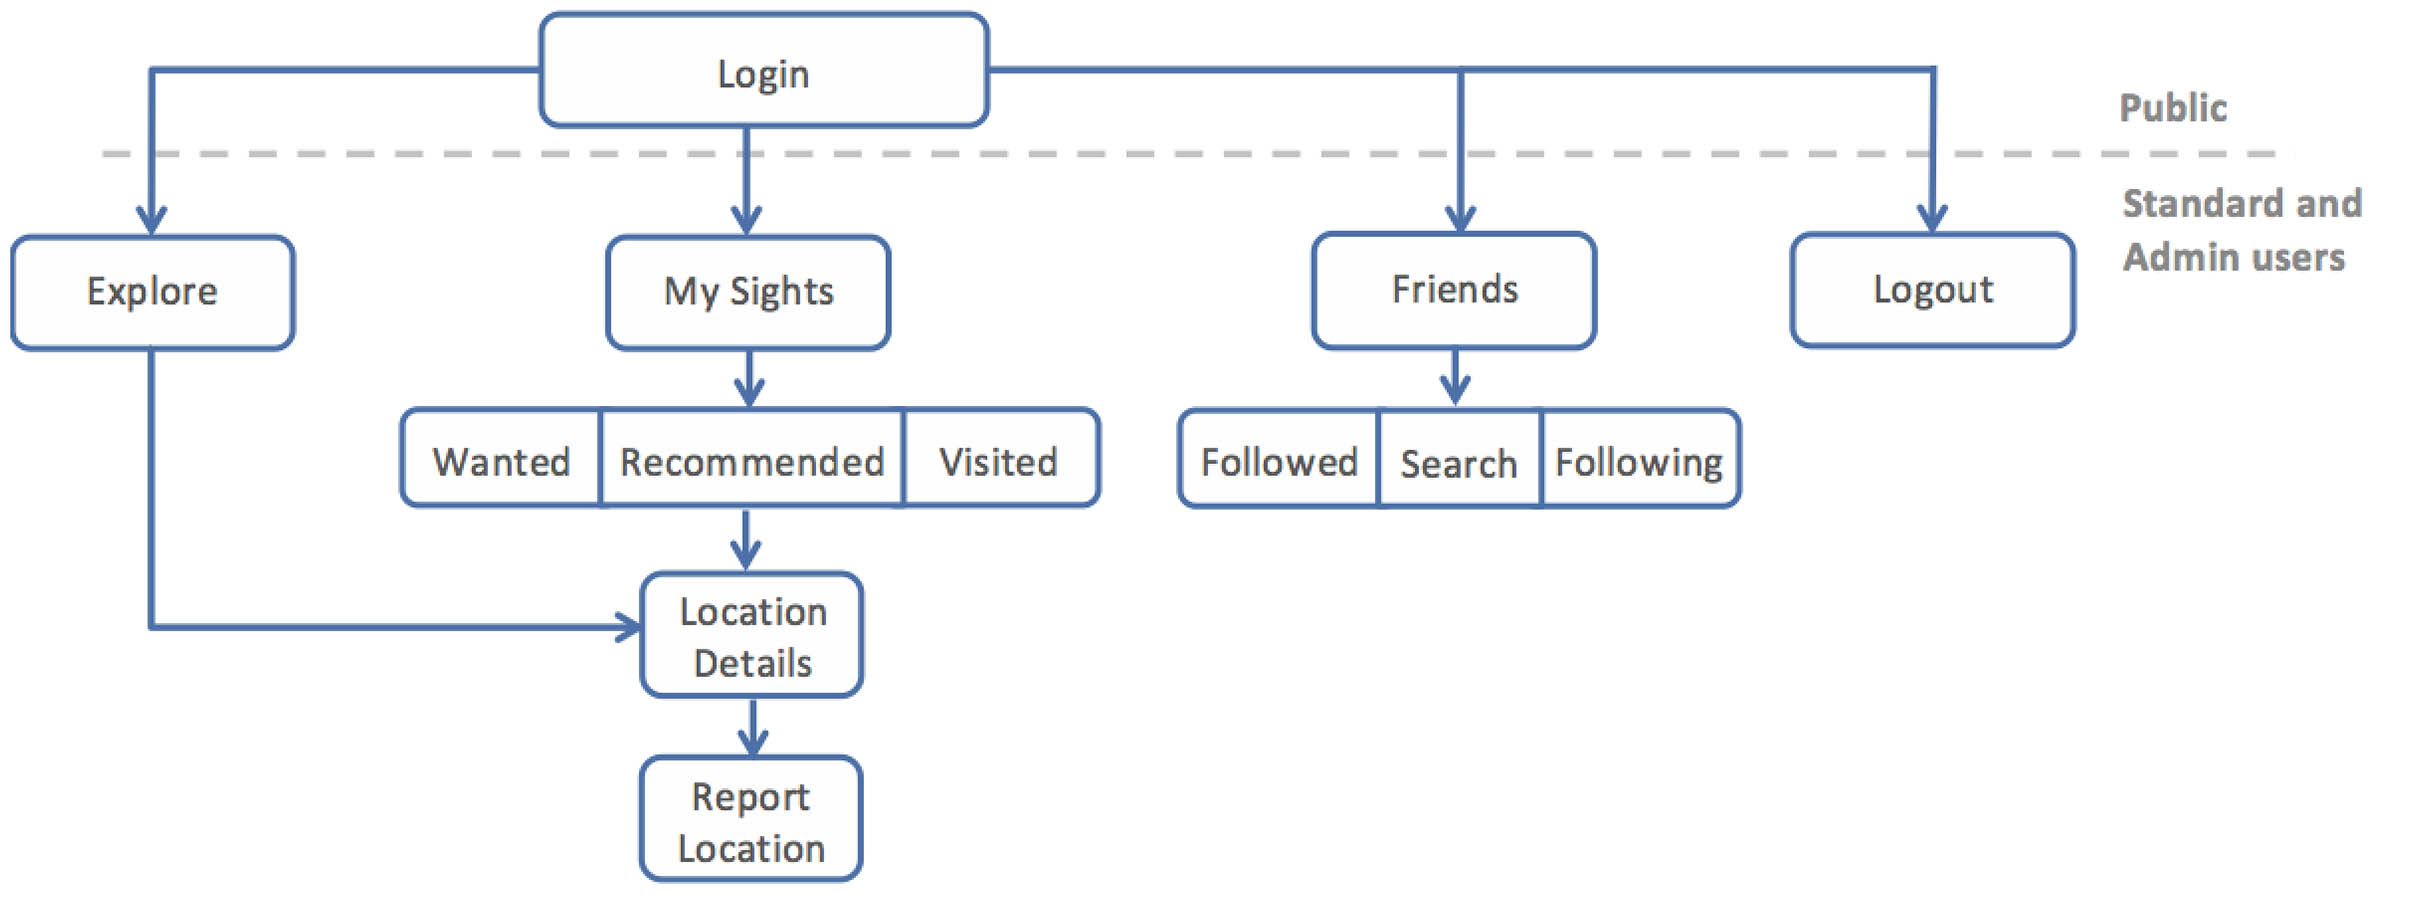
\includegraphics[height=4.4cm]{./images/diagrams/diagram_hierarchy_ios_standard.jpg}
   \caption{Operation hierarchy for the \emph{Standard} user of the iOS application.}
   \label{fig:iosStandardUserHierarchy}
\end{figure}
%%%%%%%
The \emph{Admin} users can perform the same operations as the \emph{Standard} users, as illustrated on Figure~\ref{fig:iosStandardUserHierarchy} and also some additional operations that are depicted on Figure~\ref{fig:iosAdminUserHierarchy}. The main sections of the administrative area are:
\begin{itemize}
\item Manage Sights - searching for touristic locations, edit their information or create a new touristic location.
\item Reported Sights - lists the locations that were reported by users, allowing to correct their information directly with the reported data.
\item Service Logs - allows to consult the log information from different service components.
\end{itemize}
\begin{figure}[h!]
 \centering
   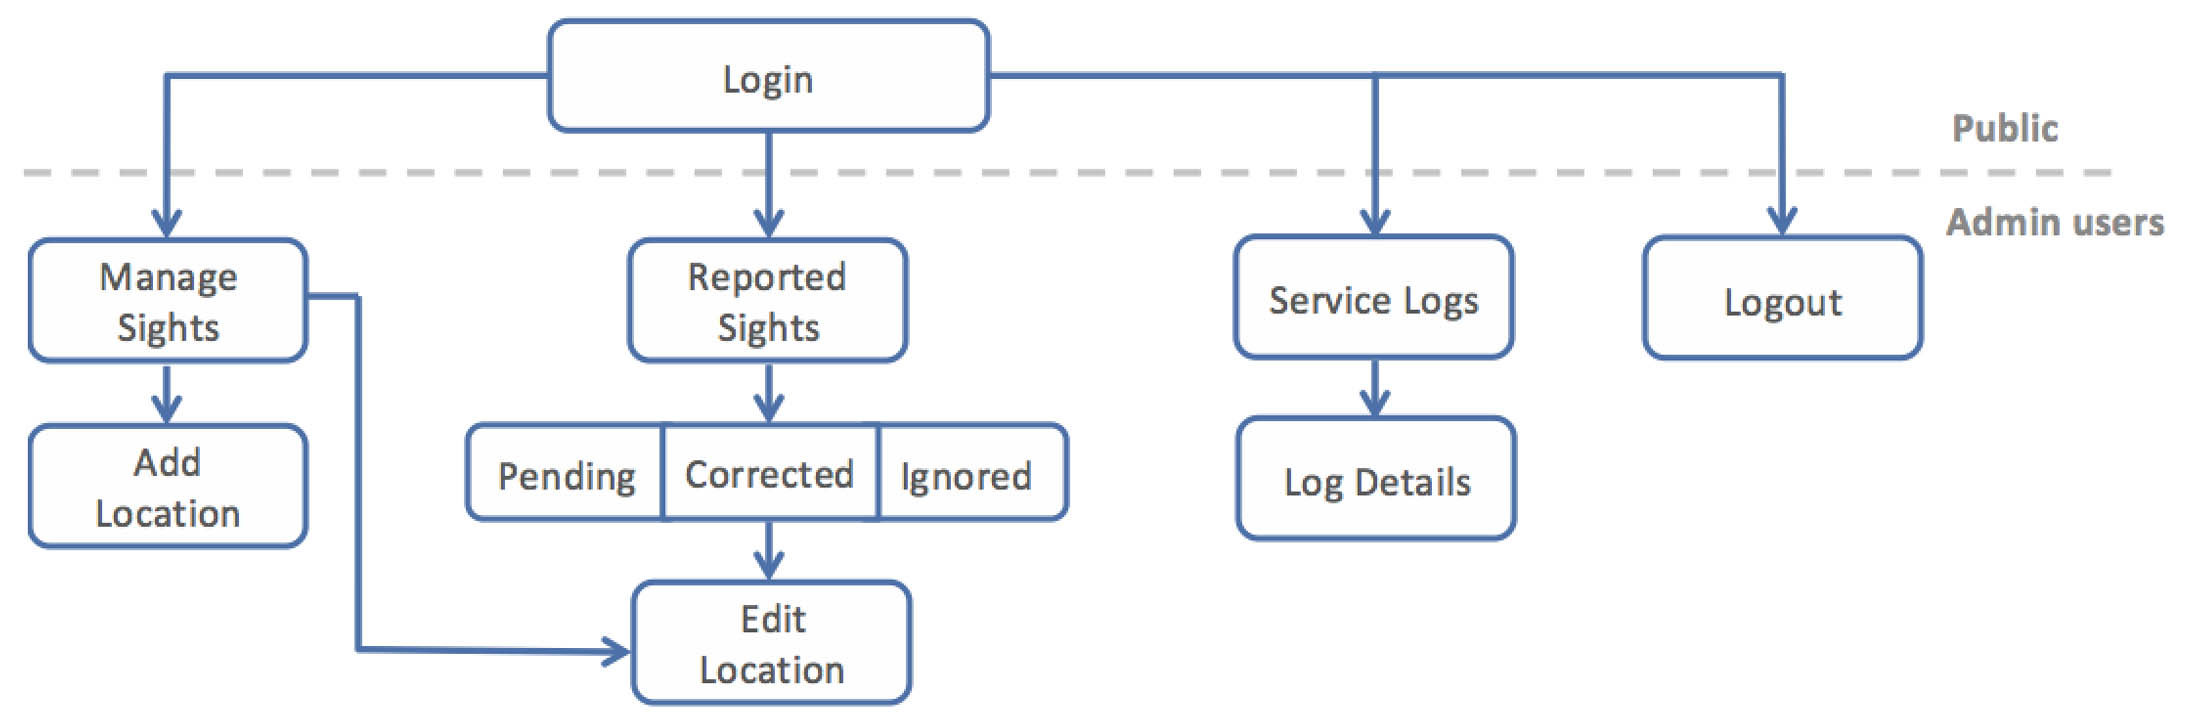
\includegraphics[height=3.8cm]{./images/diagrams/diagram_hierarchy_ios_admin.jpg}
   \caption{Operation hierarchy for the \emph{Admin} user of the iOS application.}
   \label{fig:iosAdminUserHierarchy}
\end{figure}